\section*{Βήμα 13}

Τέλος, υπολογίζουμε τους πίνακες σύγχυσης του καλύτερου μοντέλου στο validation και στο testing set.

\begin{figure}[H]
	\centering
	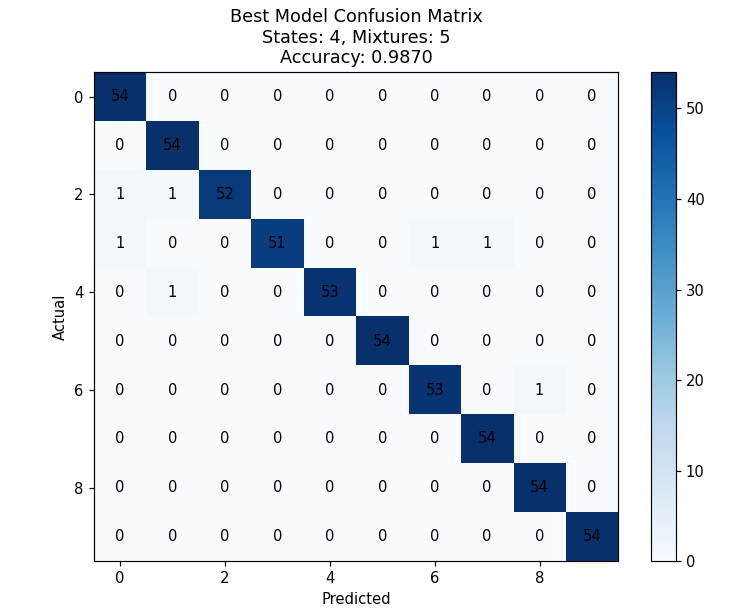
\includegraphics[width=0.8\linewidth]{../../HMM_conf_heat_validation.png}
	\caption{Πίνακας σύγχυσης του καλύτερου μοντέλου στο validation set}
\end{figure}

\begin{figure}[H]
	\centering
	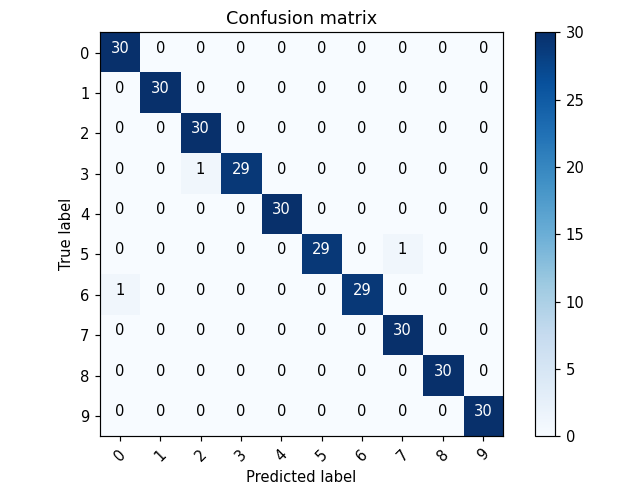
\includegraphics[width=0.8\linewidth]{../../HMM_conf_heat_testing.png}
	\caption{Πίνακας σύγχυσης στο testing set}
\end{figure}

\noindent Όπως βλέπουμε ξανά, η συνολική ακρίβεια του επιλεγμένου μοντέλου, δηλαδή το ολικό ποσοστό των σωστά κατηγοριοποιημένων εκφωνήσεων, στο testing set είναι 99\%.

\begin{figure}[H]
	\centering
	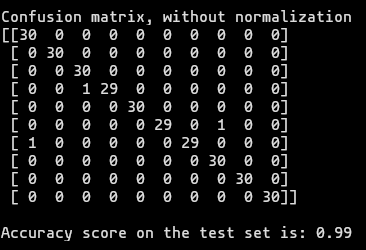
\includegraphics[width=0.5\linewidth]{../../HMM_acc_conf_testing.png}
\end{figure}